\chapter[Minimierung von FSMs$^*$]{Minimierung endlicher Automaten$^*$}
In diesem Abschnitt zeigen wir ein Verfahren, mit dem die Anzahl der Zust\"ande eines deterministischen
endlichen Automaten 
\\[0.2cm]
\hspace*{1.3cm}
$A = \langle Q, \Sigma, \delta, q_0, F \rangle$
\\[0.2cm]
minimiert werden kann.  Ohne Beschr\"ankung der Allgemeinheit wollen wir dabei voraussetzen,
dass der Automat $A$ vollst\"andig ist: Wir nehmen also an, dass der Ausdruck $\delta(q, c)$
f\"ur jeden Zustand $q \in Q$ und jeden Buchstaben $c \in \Sigma$ als Ergebnis einen Zustand
aus $Q$ liefert. Wir suchen dann einen deterministischen
endlichen Automaten 
\\[0.2cm]
\hspace*{1.3cm}
$A^- = \langle Q^-, \Sigma, \delta^-, q_0, F^- \rangle$,
\\[0.2cm]
der dieselbe Sprache akzeptiert wie der Automat $A$, f\"ur den also
\\[0.2cm]
\hspace*{1.3cm}
$L(A^-) = L(A)$
\\[0.2cm]
gilt und f\"ur den die Anzahl der Zust\"ande der Menge $Q^-$ minimal ist.  
Um diese
Konstruktion durchf\"uhren zu k\"onnen, m\"ussen wir etwas ausholen.
Zun\"achst erweitern wir die Funktion 
\\[0.2cm]
\hspace*{1.3cm}
$\delta: Q \times \Sigma \rightarrow Q$
\\[0.2cm]
zu einer Funktion $\hat{\delta}$, die als zweites Argument nicht nur einen Buchstaben
sondern auch einen String akzeptiert:
\\[0.2cm]
\hspace*{1.3cm}
$\hat{\delta} : Q \times \Sigma^* \rightarrow Q$.
\\[0.2cm]
Der Funktions-Aufruf $\hat{\delta}(q,s)$ soll den Zustand $p$ berechnen, in den der Automat $A$ gelangt,
wenn der Automat im Zustand $q$ den String $s$ liest.
Die Definition von $\hat{\delta}(q,s)$ erfolgt durch Induktion \"uber die L\"ange des Strings $s$:
\begin{enumerate}
\item[I.A.:] $\hat{\delta}(q,\varepsilon) = q$,
\item[I.S.:] $\hat{\delta}(q,cs) = \hat{\delta}\bigl(\delta(q,c),s\bigr)$, 
             falls $c \in   \Sigma$ und $s \in \Sigma^*$.
\end{enumerate}
Da die Funktion $\hat{\delta}$ eine Verallgemeinerung der Funktion $\delta$ ist, werden wir in der
Notation nicht zwischen $\delta$ und $\hat{\delta}$ unterscheiden und einfach nur $\delta$ schreiben.

Offensichtlich k\"onnen wir in einem endlichen Automaten 
$A = \langle Q, \Sigma, \delta, q_0, F \rangle$  alle die Zust\"ande $p \in Q$ entfernen,
die vom Start-Zustand aus nicht 
\emph{erreichbar} sind.  Dabei hei{\ss}t ein Zustand $p$ \emph{erreichbar} genau dann, wenn es
einen String $w \in \Sigma^*$ gibt, so dass
\\[0.2cm]
\hspace*{1.3cm}
$\delta(q_0, w) = p$
\\[0.2cm]
gilt.  Wir wollen im Folgenden daher voraussetzen, dass alle Zust\"ande des betrachteten
endlichen Automaten vom Start-Zustand aus erreichbar sind.


\begin{figure}[!ht]
  \centering
  \epsfig{file=Abbildungen/nicht-gleichwertig.eps, scale=0.6}
   \caption{Ein endlicher Automat mit \"aquivalenten Zust\"anden.}
  \label{fig:nicht-gleichwertig.dot}
\end{figure}

Im Allgemeinen k\"onnen wir einen Automaten dadurch minimieren, dass wir bestimmte Zust\"ande
identifizieren.  Betrachten wir beispielsweise den in Abbildung
\ref{fig:nicht-gleichwertig.dot} gezeigten Automaten, so k\"onnen wir dort die Zust\"ande $q_1$
und $q_2$ sowie $q_3$ und $q_4$ identifizieren, ohne dass sich dadurch die Sprache des
Automaten \"andert.  
Die zentrale Idee bei der Minimierung eines Automaten besteht darin, dass wir uns
\"uberlegen, welche Zust\"ande wir auf keinen Fall identifizieren d\"urfen und einfach alle
anderen Zust\"ande als \"aquivalent betrachten.

\begin{Definition}[Separable States]
Assume $A = \langle Q, \Sigma, \delta, q_0, F \rangle$ is a deterministic finite state machine.
Two states $p_1,p_2 \in Q$ are called \emph{separable} if and only if there exists a string 
$s \in \Sigma^*$ such that either
\begin{enumerate}
\item $\delta(p_1,s) \in    F$ and $\delta(p_2,s) \notin F$ or
\item $\delta(p_1,s) \notin F$ and $\delta(p_2,s) \in    F$
\end{enumerate}
holds.  In this case, the string $s$ \emph{separates} $p_1$ and $p_2$. \qed
\end{Definition}
If two states $p_1$ and $p_2$ are separable, then it is obvious that theses states are not
equivalent.
We define an equivalence relation $\sim$ on the set $Q$ of all states by setting
\\[0.2cm]
\hspace*{1.3cm}
$p_1 \sim p_2$ \quad iff \quad 
$\forall s \in \Sigma^*:\bigl(\delta(p_1,s) \in F \leftrightarrow \delta(p_2,s) \in F\bigr)$.
\\[0.2cm]
Hence, two states $p_1$ and $p_2$ are considered to be equivalent iff they are not separable.   
The claim is that we can identify all equivalent states.  The identification of two states $p_1$ and
$p_2$ is done by removing the state $p_2$ from the set $Q$ and changing the transition
function $\delta$ in a way that the new version of $\delta$ will return
$p_1$ in all those cases where the old version of $\delta$ had returned $p_2$.


Es bleibt die Frage zu kl\"aren, wie wir feststellen k\"onnen, welche Zust\"ande unterscheidbar sind.
Eine M\"oglichkeit besteht darin, eine Menge $V$ von Paaren von Zust\"ande anzulegen.  Wir f\"ugen
das Paar $\langle p, q \rangle$ in die Menge $V$ ein, wenn wir erkannt haben, dass $p$ und $q$
unterscheidbar sind.  Wir erkennen $p$ und $q$ als unterscheidbar, wenn es einen Buchstaben 
$c\in\Sigma$ und zwei Zust\"ande $s$ und $t$ gibt, so dass 
\\[0.2cm]
\hspace*{1.3cm}
$\delta(p,c) = s$, $\delta(q,c) = t$ und $\langle s, t \rangle \in V$
\\[0.2cm]
gilt.  Diese Idee liefert einen Algorithmus, der aus zwei Schritten besteht:
\begin{enumerate}
\item Zun\"achst initialisieren wir $V$ mit alle den Paaren $\pair(p,q)$, f\"ur die entweder
      $p$ ein akzeptierender Zustand und $q$ kein akzeptierender Zustand ist, oder
      umgekehrt $q$ ein akzeptierender Zustand und $p$ kein akzeptierender Zustand ist,
      denn ein akzeptierender Zustand kann durch den leeren String $\varepsilon$ von einem
      nicht-akzeptierenden Zustand unterschieden werden:
      \\[0.2cm]
      \hspace*{1.3cm}
      $V := \bigl\{\pair(p,q) \in Q \times Q \mid (p \in F \wedge q \notin F) \vee 
                                               (p \notin F \wedge q \in F) \bigr\}$
\item Solange wir ein neues Paar $\pair(p,q) \in Q \times Q$ finden, f\"ur dass es einen 
      Buchstaben $c$ gibt, so dass die Zust\"ane $\delta(p,c)$ und $\delta(q,c)$ 
      bereits unterscheidbar sind, f\"ugen wir dieses Paar zur Menge $V$ hinzu: 
      \\[0.2cm]
      \hspace*{1.3cm} 
      \texttt{while ($\exists \pair(p,q) \in Q \times Q: \exists c \in \Sigma:\langle\delta(p,c),
        \delta(q,c)\rangle \in V \wedge \pair(p,q) \notin V$) \{} \\
      \hspace*{1.8cm}
      \texttt{choose $\pair(p,q) \in Q \times Q$ such that} $\langle\delta(p,c),
      \delta(q,c)\rangle \in V \wedge \pair(p,q) \notin V$ \texttt{\{}
\\
      \hspace*{2.3cm}
      \texttt{$V$ := $V \cup \{\, \pair(p,q),\, \pair(q,p)\, \}$;} \\
      \hspace*{1.8cm}
      \texttt{\}}\\
      \hspace*{1.3cm}
      \texttt{\}}
\end{enumerate}
Haben wir alle Paare $\pair(p,q)$ von unterscheidbaren Zust\"anden gefunden,
so k\"onnen wir anschlie{\ss}end alle Zust\"ande $p$ und $q$  identifizieren, die nicht
unterscheidbar sind, f\"ur die also $\langle p, q \rangle \not\in V$ gilt.
Es l\"asst sich zeigen, dass der so konstruierte Automat tats\"achlich minimal ist.
\pagebreak

\vspace*{-0.5cm}
\example
Wir betrachten den in Abbildung \ref{fig:nicht-gleichwertig.dot} gezeigten endlichen
Automaten und wenden den oben skizzierten Algorithmus auf diesen Automaten an.
Wir bedienen uns dazu einer Tabelle, deren Spalten und Zeilen mit den verschiedenen
Zust\"anden durchnummeriert sind.  Wenn wir im ersten Schritt erkannt haben,
dass die Zust\"ande $i$ und $j$ unterscheidbar sind, so f\"ugen wir in dieser Tabelle
 in der $i$-ten Zeile und der $j$-ten Spalte eine $1$ ein.
Da mit den Zust\"anden $i$ und $j$ auch die Zust\"ande $j$ und $i$ unterscheidbar sind,
f\"ugen wir au{\ss}erdem in der $j$-ten Zeile und der $i$-ten Spalte ebenfalls eine $1$ ein.
\begin{enumerate}
\item Im ersten Schritt erkennen wir, dass die beiden akzeptierenden Zust\"ande
      $q_3$ und $q_4$ von allen nicht-akzeptierenden Zust\"anden unterscheidbar sind.
      Also sind die Paare 
      $\pair(q_0,q_3)$,
      $\pair(q_0,q_4)$,
      $\pair(q_1,q_3)$,
      $\pair(q_1,q_4)$,
      $\pair(q_2,q_3)$ und
      $\pair(q_2,q_4)$
      unterscheidbar.  Damit hat die Tabelle nun die folgende Gestalt:
      \begin{center}        
      \begin{tabular}[t]{|l||l|l|l|l|l|}
      \hline
            & $q_0$    &    $q_1$ &    $q_2$ &      $q_3$ &      $q_4$  \\
      \hline
      \hline
      $q_0$ &          &          &          & $1$ & $1$  \\
      \hline
      $q_1$ &          &          &          &$1$ &$1$  \\
      \hline
      $q_2$ &          &          &          &$1$ &$1$  \\
      \hline
      $q_3$ &$1$        &$1$         &       $1$ &          &           \\
      \hline
      $q_4$ &$1$ &$1$ &$1$ &          &           \\
      \hline
      \end{tabular}
      \end{center}
\item Als n\"achstes erkennen wir, dass die Zust\"ande $q_0$ und $q_1$ unterscheidbar sind,
      denn es gilt 
      \\[0.2cm]
      \hspace*{1.3cm}
      $\delta(q_0,a) = q_1$, \quad $\delta(q_1,a) = q_3$ \quad und \quad $q_1 \not\sim q_3$.
      \\[0.2cm]
      Genauso sehen wir, dass die Zust\"ande $0$ und $2$ unterscheidbar sind, 
      denn es gilt 
      \\[0.2cm]
      \hspace*{1.3cm}
      $\delta(q_0,b) = q_2$, \quad $\delta(q_2,b) = q_4$ \quad und \quad $q_2 \not\sim q_4$.
      \\[0.2cm]
      Da wir im zweiten Schritt nun gefunden haben, dass
      $q_0 \not\sim q_1$ und $q_0 \not\sim q_2$ gilt, tragen wir in der Tabelle an den
      entsprechenden Stellen eine $2$ ein. Damit hat die Tabelle
      jetzt die folgende Gestalt:
      \begin{center}        
      \begin{tabular}[t]{|l||l|l|l|l|l|}
      \hline
        & $q_0$      &      $q_1$ &      $q_2$ &      $q_3$ &      $q_4$  \\
      \hline
      \hline
      $q_0$ &          &$2$ &$2$ &$1$ &$1$  \\
      \hline
      $q_1$ &$2$ &          &          &$1$ &$1$  \\
      \hline
      $q_2$ &$2$ &          &          &$1$ &$1$  \\
      \hline
      $q_3$ &$1$ &$1$ &$1$ &          &           \\
      \hline
      $q_4$ &$1$ &$1$ &$1$ &          &           \\
      \hline
      \end{tabular}
      \end{center}
\item Nun finden wir keine weiteren Paare von unterscheidbaren Zust\"anden mehr,
      denn wenn wir das Paar $\pair(q_1,q_2)$ betrachten, sehen wir
      \\[0.2cm]
      \hspace*{1.3cm}
      $\delta(q_1,\texttt{a}) = q_3$ \quad und \quad $\delta(q_2,\texttt{a}) = q_4$, 
      \\[0.2cm]
      aber da die Zust\"ande $3$ und $4$ bisher nicht unterscheidbar sind,
      liefert dies kein neues unterscheidbares Paar.  Genausowenig liefert
      \\[0.2cm]
      \hspace*{1.3cm}
      $\delta(q_1,\texttt{b}) = q_3$ \quad und \quad $\delta(q_2,\texttt{b}) = q_4$, 
      \\[0.2cm]
      ein neues unterscheidbares Paar.  Jetzt bleiben noch die beiden Zust\"ande
      $q_3$ und $q_4$.  Hier finden wir
      \\[0.2cm]
      \hspace*{1.3cm}
      $\delta(q_3,c) = q_1$ \quad und \quad $\delta(q_4,c) = q_2$ \quad f\"ur alle $c \in \{\texttt{a}, \texttt{b}\}$
      \\[0.2cm]
      und da die Zust\"ande $q_1$ und $q_2$ bisher nicht als unterscheidbar bekannt sind,
      haben wir keine neuen unterscheidbaren Zust\"ande gefunden.
      Damit k\"onnen wir die \"aquivalenten Zust\"ande aus der Tabelle ablesen, es gilt:
      \begin{enumerate}
      \item $q_1 \sim q_2$
      \item $q_3 \sim q_4$
      \end{enumerate}
      Abbildung \ref{fig:gleichwertig.dot} zeigt den entsprechenden reduzierten endlichen
      Automaten.
\end{enumerate}

\begin{figure}[!ht]
  \centering
  \epsfig{file=Abbildungen/gleichwertig.eps, scale=0.6}
   \caption{Der reduzierte endliche Automat.}
  \label{fig:gleichwertig.dot}
\end{figure}



\exercise
Konstruieren Sie den minimalen deterministischen endlichen Automaten, der die Sprache \linebreak
$L\bigl(a \cdot (b \cdot a)^*\bigr)$ erkennt.  Gehen Sie dazu in folgenden Schritten vor:
\begin{enumerate}
\item[(a)] Berechnen Sie einen nicht-deterministischen endlichen Automaten, der diese Sprache
           erkennt.
\item[(b)] Transformieren Sie diesen Automaten in einen deterministischen Automaten.
\item[(c)] Minimieren Sie die Zahl der Zust\"ande dieses Automaten mit dem oben angegebenen Algorithmus.
\end{enumerate}

\section{Implementing  the Minimization  of Finite Automata in \textsc{SetlX}}
Figure \ref{fig:minimize.stlx} on page \pageref{fig:minimize.stlx} shows the function
\texttt{minimize} that takes a determininistic finite state machine \texttt{fa} as input.
The function eliminates all states from \texttt{fa} that are not reachable from the start
state and then tries to minimize equivalent states as discussed in the previous section.
It returns a finite state machine that accepts the same language as \texttt{fa} and that,
furthermore, is guaranteed to have as few states as possible.  The implementation works as
discussed below.

\begin{figure}[!ht]
\centering
\begin{Verbatim}[ frame         = lines, 
                  framesep      = 0.3cm, 
                  firstnumber   = 1,
                  labelposition = bottomline,
                  numbers       = left,
                  numbersep     = -0.2cm,
                  xleftmargin   = 0.5cm,
                  xrightmargin  = 0.5cm,
                ]
    minimize := procedure(fa) {
        [states, sigma, delta, q0, accepting] := fa;
        states    := fixpoint( {q0}, q |=> { delta[q, c] : c in sigma });
        separable := (states-accepting) >< accepting + accepting >< (states-accepting);
        moreSep   := 
            procedure(knownSep) {
                return { [q1, q2] : [q1, q2] in states >< states
                       | exists (c in sigma | [delta[q1, c], delta[q2, c]] == knownSep)
                       };
            };
        allSeparable := fixpoint(separable, moreSep);
        equivalent   := states >< states - allSeparable;
        equivClasses := { { p : p in states | [p, q] in equivalent }: q in states };
        newQ0        := arb({ m : m in equivClasses | q0 in m });
        newAccept    := { m : m in equivClasses | arb(m) in accepting };   
        newDelta     := {};
        for (q in states, c in sigma) {
            p := delta[q, c];
            if (p != om) {
                classOfP := findEquiv(p, equivClasses);
                classOfQ := findEquiv(q, equivClasses);
                newDelta += { [[classOfQ, c], classOfP] };
            }
        }
        return [equivClasses, sigma, newDelta, newQ0, newAccept];
    };
    findEquiv := procedure(p, eqClasses) {
        return first({ cl : cl in eqClasses | p in cl });
    };
\end{Verbatim}
\vspace*{-0.3cm}
\caption{A procedure to minimize a finite state machine.}
\label{fig:minimize.stlx}
\end{figure}

\begin{enumerate}
\item First, all states \emph{reachable} from the start state $q_0$ are computed.
      Here, a state $p$ is \emph{reachable} from the state $q_0$ iff there is a string $s$
      such that $\delta(q_0, s) = p$.
      The computation of the reachable states is done via a fixpoint computation:
      \begin{enumerate}
      \item Since $\delta(q_0, \varepsilon) = q_0$, the state $q_0$ is reachable from $q_0$
            and therefore we initialize the set \texttt{reachable} with the 
            start state $q_0$.
      \item The remaining reachable states are found by a fixpoint iteration.
            Given a state $q$, the function
            \\[0.2cm]
            \hspace*{1.3cm}
            \texttt{q |=> \{ delta(q, c) : c in sigma \}}
            \\[0.2cm]
            computes the set of all states reachable from $q$ by reading some letter $c \in \Sigma$.

            Using the second order function \texttt{fixpoint} discussed in the previous chapter in
            Figure \ref{fig:nfa2dfa.stlx} on page \pageref{fig:nfa2dfa.stlx}, the set of all
            states reachable from $q_0$ is then found by iterating the function 
            \\[0.2cm]
            \hspace*{1.3cm}
            \texttt{q |=> \{ delta(q, c) : c in sigma \}}
            \\[0.2cm]
            until no new states are found.
      \end{enumerate}
\item Next, we try to find all pairs of states that are \emph{separable}. Remember, 
      a pair $\pair(p, q)$ is called \emph{separable} if there is a string $s$ such
      that either $\delta(p,s)$ is accepting while $\delta(q,s)$ is not accepting, or
      $\delta(p,s)$ is not accepting while $\delta(q,s)$ is accepting.  
      \begin{enumerate}
      \item Initially, we know that a pair $\pair(p, q)$ is separable if either
            $p$ is a member of the set \texttt{accepting} of accepting states while $q$
            is not a member of \texttt{accepting} or it is the other way around:
            $p \not\in \mathtt{accepting}$ and $q \in \mathtt{accepting}$.

            Therefore, the set \texttt{separable} is initialzed as the set
            \\[0.2cm]
            \hspace*{1.3cm}
            $(\mathtt{states}\backslash \mathtt{accepting}) \times \mathtt{accepting} \cup
             \mathtt{accepting} \times (\mathtt{states}\backslash \mathtt{accepting})  
            $.
            \\[0.2cm]
            This expression is coded in \textsc{SetlX} in line 4.  Note that
            the set difference $a \backslash b$ of two sets $a$ and $b$ is written as
            $a \texttt{-} b$ in \textsc{SetlX}, while the \emph{cartesian product} 
            $a \times b$ of $a$ and $b$ is written as $a \texttt{><} b$.  Remember that the
            cartesian product of two sets $a \times b$ is defined as 
            \\[0.2cm]
            \hspace*{1.3cm}
            $a \times b := \{ \pair(x,y) \mid x \in a \wedge y \in b \}$.
      \item Next, if the states $\delta(q_1,c)$ and $\delta(q_2,c)$ are already known
            to be separable, then the states $q_1$ and $q_2$ are also separable.  The
            reasoning is as follows:  As $\delta(q_1,c)$ and $\delta(q_2,c)$ are separable,
            there is a string $s$ such that
            \\[0.2cm]
            \hspace*{1.3cm}
            $\delta(\delta(q_1,c), s)$ is accepting \quad while \quad
            $\delta(\delta(q_2,c), s)$ is not accepting 
            \\[0.2cm]
            or the other way arround.  As we have $\delta(\delta(q_1,c), s) = \delta(q_1, cs)$
            and $\delta(\delta(q_2,c), s) = \delta(q_2, cs)$ this can be rewritten as
            \\[0.2cm]
            \hspace*{1.3cm}
            $\delta(q_1,cs)$ is accepting \quad while \quad
            $\delta(q_2,cs)$ is not accepting
            \\[0.2cm]
            or the other way around.  
            By the definition of two states being separable 
            this implies that $q_1$ and $q_2$ are separable. 
            Hence, the set of all pairs of separable states can be found by a fixpoint
            iteration. 
            The procedure \texttt{moreSep} defined in line 5 takes a pair of states
            \texttt{knownSep} that are already known to be separable.  For any pair of states
           $\langle q_1, q_2 \rangle$ and any character $c \in \Sigma$ it then checks whether the pair
           \\[0.2cm]
           \hspace*{1.3cm}
           $\langle \delta(q_1,c), \delta(q_2, c) \rangle$
           \\[0.2cm]
           equals the pair \texttt{knownSep}, because then $\langle q_1, q_2 \rangle$ is separable,
           too.  Using this function, the set of all separable pairs can then be computed via a
           straightforward fixpoint iteration in line 11.

           I have to admit that the current implementation of the separable states could be done 
           more efficiently.  However, this would have complicated the program and for the purpose 
           of the examples presented in this lecture the efficiency is sufficient.
      \end{enumerate}
\item Next, we \emph{identify} those states that are \emph{equivalent}: Two states
      $p$ and $q$ are called \emph{equivalent} if and only if they are
      \underline{not} separable.  
 
      There are several way to identify equivalent states.  The easiest way is to compute
      the associated \emph{equivalence classes}, where an equivalence class contains all
      thoses states that are equivalent to each other.
      \begin{enumerate}
      \item Therefore, the set of states of the minimized finite state machine is the set
            of equivalence classes of states of the given finite state machine
            \texttt{fa}.   For example, if the set of states of \texttt{fa} is
            \\[0.2cm]
            \hspace*{1.3cm}
            \texttt{\{ $q_0$, $q_1$, $q_2$, $q_3$, $q_4$, $q_5$ \}}
            \\[0.2cm]
            and the state $q_1$ is equivalent to  $q_2$ and, furthermore, the states
            $q_3$, $q_4$, and $q_5$ are pairwise equivalent, then the set of equivalence
            classes is given as
            \\[0.2cm]
            \hspace*{1.3cm}
            \texttt{\{ \{$q_0$\}, \{$q_1$, $q_2$\}, \{$q_3$, $q_4$, $q_5$\} \}}.
            \\[0.2cm]
            This set of equivalence classes is the new set of states.
      \item Of course, the new start state is the set of equivalent states that contains
            the start state $q_0$ of the given finite state machine \texttt{fa}.
            In line 14 we collect the set of all equivalence classes that contain \texttt{q0}.
            Of course, there can be just one equivalence class.  Hence we can extract this one
            class using the function \texttt{arb}.
      \item A set of equivalent states is accepting if any of its member states is an
            accepting state.  Of course, if a set of equivalent states contains an
            accepting state, then the other states in this equivalence class have to be
            accepting also, since otherwise these states would be separable from the
            accepting state and therefore could not be equivalent.
      \end{enumerate}
\item In order to compute the new state transition function, we have to construct a
      function that takes a set of equivalent states of the old finite state machine
      \texttt{fa} and turns this set into a new set of states that are again
      equivalent.  This is done by taking all states \texttt{q} and all characters \texttt{c} 
      in \texttt{sigma} and computing 
      \\[0.2cm]
      \hspace*{1.3cm}
      $\mathtt{p} = \delta(\mathtt{q}, \mathtt{c})$.
      \\[0.2cm]
      Now, if \texttt{classOfQ} is the equivalence class containing \texttt{q} and likewise 
      \texttt{classOfP} is the equivalence class containing \texttt{p}, then we have
      \\[0.2cm]
      \hspace*{1.3cm}
      $\texttt{classOfP} = \texttt{newDelta}(\texttt{classOfQ}, \texttt{c})$.
      \\[0.2cm]
      Here, \texttt{newDelta} is the transition function of the minimized finite state machine.
\end{enumerate}

\section{The Theorem of Nerode}
A language is called a \emph{regular} language iff there is a finite state machine $A$
recognizing the language.  We have already seen that a language is regular iff it is
accepted by a finite state machine.
In this section we discuss a theorem that can be used to prove that a given language is
\underline{not} a regular language.  The main idea is to extend the
notion of \emph{separability} from states to strings.

\begin{Definition}[separable]
  Given an alphabet $\Sigma$ and a formal language $L \subseteq \Sigma^*$, a pair of strings
  $\pair(s,t) \in \Sigma^* \times \Sigma^*$ is called 
  \emph{separable with respect to $L$} iff there is a string $w \in \Sigma^*$ 
  such that 
  \\[0.2cm]
  \hspace*{1.3cm}
  $(sw \in L \,\wedge\, tw \not\in L) \,\vee\, (sw \not\in L \,\wedge\, tw \in L)$.  
  \\[0.2cm]
  In this case, $w$ is the \emph{witness of the separability} of $\pair(s,t)$.
  If the pair $\pair(s,t)$ is separable with respect to $L$ and if the language $L$ is
  obvious from the context, then in order to shorten our notation, we call $s$ and $t$
  separable.
  \qed
\end{Definition}
\pagebreak

\exampleEng
 Take $\Sigma = \{ \mathtt{a}, \mathtt{b} \}$ and define $L$ as the
language of all strings of the form $a^nb^n$ where $n$ is a natuaral number, i.~e.~define
\\[0.2cm]
\hspace*{1.3cm}
$L := \{ \mathtt{a}^n\mathtt{b}^n \mid n \in \mathbb{N} \}$.
\\[0.2cm]
Then the strings $s := \texttt{aaab}$ and $t := \texttt{bba}$ are separable and
$w := \mathtt{bb}$ is a witness of separability because
\\[0.2cm]
\hspace*{1.3cm}
$sw = \mathtt{aaabbb} \in L$ \quad but \quad $tw = \mathtt{bbabb} \not\in L$.  \eox

\exerciseEng
Assume $\Sigma$ is an alphabet and $L \subseteq \Sigma^*$ is a formal language.  Define a
relation $\sim_L$ on $\Sigma^*$ as follows:
\\[0.2cm]
\hspace*{1.3cm}
$s_1 \sim_L s_2$ 
\quad iff \quad $s_1$ and $s_2$ are \underline{not} separable with respect to $L$.
\\[0.2cm]
Prove that the relation $\sim_L$ is an equivalence relation!  \eox
\vspace*{0.3cm}


\noindent
The following theorem has been proven by Anil Nerode in 1958 \cite{nerode:58}. 
It can be used to show that certain languages are not regular.

\begin{Theorem}[Nerode]
  If $L \subseteq \Sigma^*$ is a formal language and $S = \{ s_1, \cdots, s_n \} \subseteq \Sigma^*$
  is a set of strings that are pairwise separable with respect to $L$ and, furthermore, $A$ is a 
  determininistic finite state machine recognizing the language $L$, then
  $A$ has at least $n$ different states.
\end{Theorem}

\proofEng
Assume $A = \langle Q, \Sigma, \delta, q_0, F\rangle$ is a \textsc{Dfa}  accepting the
language $L$, i.~e.~$L(A) = L$.  Define states
\\[0.2cm]
\hspace*{1.3cm}
$q_i := \delta(q_0, s_i)$ \quad for all $i \in \{ 1,\cdots,n \}$.
\\[0.2cm]
The claim is that all these states are pairwise different, that is we have
\\[0.2cm]
\hspace*{1.3cm}
$\forall i,j \in \{ 1, \cdots, n \}: i \not=j \rightarrow q_i \not= q_j$.
\\[0.2cm]
Therefore, assume that we have $i \not= j$.  
By our assumption, the strings $s_i$ and $s_j$ are separable.  Then there is a
witness $w \in \Sigma^*$ such that
\\[0.2cm]
\hspace*{1.3cm}
$(s_iw \in L \,\wedge\, s_jw \not\in L) \vee (s_iw \not\in L \,\wedge\, s_jw \in L)$.
\\[0.2cm]
These are two cases which we consider separately.
\begin{enumerate}
\item $s_iw \in L \,\wedge\, s_jw \not\in L$.

      Since the \textsc{Dfa} $A$ accepts the language $L$, we know that
      \\[0.2cm]
      \hspace*{1.3cm}
      $\delta(q_0, s_iw) \in F \;\wedge\; \delta(q_0, s_jw) \not\in F$.
      \\[0.2cm]
      On the other hand, we have
      \\[0.2cm]
      \hspace*{1.3cm}
      $\delta(q_0, s_iw) = \delta(\delta(q_0, s_i), w) = \delta(q_i, w)$ \quad and \quad
      $\delta(q_0, s_jw) = \delta(\delta(q_0, s_j), w) = \delta(q_j, w)$.
      \\[0.2cm]
      From this we can conclude
      \\[0.2cm]
      \hspace*{1.3cm}
      $\delta(q_i, w) \in F \;\wedge\; \delta(q_j, w) \not\in F$.
      \\[0.2cm]
      This is only possible if $q_i \not= q_j$.
\item $s_iw \not\in L \,\wedge\, s_jw \in L$.

      If we exchange the roles of $i$ and $j$, this case is reduced to the previous case
      and we can again conclude that $q_i \not= q_j$.
\end{enumerate}
We have just shown that $q_i \not= q_j$ as long as $i \not= j$.  Therefore the states
$\{ q_1, \cdots, q_n \}$ are all pairwise different and the finite state machine $A$ needs
to have at least $n$ different states.
\qed
\pagebreak

\begin{Corollary}
If $L \subseteq \Sigma^*$ is a formal language such that for every natural number $n \in \mathbb{N}$
there is a set of states $\{ s_1, \cdots, s_n \}$ that are pairwise separable with respect to $L$,
then $L$ is not regular. 
\end{Corollary}

\proofEng
The proof of this claim is indirect.  Assume that $L$ is regular.  Then there is a finite state machine
\\[0.2cm]
\hspace*{1.3cm}
$F = \langle Q, \Sigma, \delta, q_0, A \rangle$
\\[0.2cm]
such that $L = L(F)$.  Define $n := \textsl{card}(Q) + 1$
where $\textsl{card}(Q)$ denotes the number of elements of $Q$.  By our assumption, there is a set
of strings $\{ s_1, \cdots, s_n \}$ that are pairwise separable.  By the theorem of
Nerode the finite state machine $F$ must then have at least $n = \textsf{card}(Q) +1$ states,
contradicting the fact that $F$ has only $\textsl{card}(Q)$ states.
\qed


\exampleEng
We prove that the language 
\\[0.2cm]
\hspace*{1.3cm}
$L := \{ \mathtt{a}^k\mathtt{b}^k \mid k \in \mathbb{N} \}$
\\[0.2cm]
is not regular.  The proof is done by contradiction.  Assume $L$ is regular.  Then there
is a \textsc{Dfa} 
\\[0.2cm]
\hspace*{1.3cm}
$A := \langle Q, \Sigma, \delta, q_0, F \rangle$ 
\\[0.2cm]
that recognizes $L$. Next, pick an arbitrary natural number $n$ and consider the following
set of strings: 
\\[0.2cm]
\hspace*{1.3cm}
$S := \{ \mathtt{a}^1,\, \mathtt{a}^2,\, \cdots,\, \mathtt{a}^n \}$.
\\[0.2cm]
$S$ contains $n$ strings and we claim that these strings are all pairwise separable.
In order to see this, take $i,j \in \{ 1,\cdots,n \}$ such that $i \not= j$ and consider
the strings $\mathtt{a}^i$ and $\mathtt{a}^j$.  The witness $\mathtt{b}^i$ separates these
strings because
\\[0.2cm]
\hspace*{1.3cm}
$\mathtt{a}^i\mathtt{b}^i \in L$ \quad but \quad $\mathtt{a}^j\mathtt{b}^i \not\in L$
\\[0.2cm]
since $j \not= i$.  Since $n$ was arbitrary, the corollary to the theorem of Nerode now shows that
the language $L$ can not be a regular language. 
\qed

\exerciseEng
Prove that the language
\\[0.2cm]
\hspace*{1.3cm}
$\{ \mathtt{a}^{k^2} \mid k \in \mathbb{N} \}$
\\[0.2cm]
is not regular.  \eox
\vspace*{0.2cm}

\noindent
\textbf{Hint}: Use the fact that the gap between the two successive square numbers $k^2$ and $(k+1)^2$
has size $2 \cdot k + 1$.


\exerciseEng
Prove that the language
\\[0.2cm]
\hspace*{1.3cm}
$\{ \mathtt{a}^{p} \mid p \in \mathbb{N} \wedge \mbox{$p$ is prime} \}$
\\[0.2cm]
is not regular.  
\vspace*{0.2cm}

\noindent
\textbf{Hint}:  It is known that the number of primes is infinite and that there are
\href{http://en.wikipedia.org/wiki/Prime_gap#Simple_observations}{gaps} of arbitrary size between
the prime numbers, so given an arbitrary natural number 
$k$, there is a pair of primes $\pair(p_1, p_2)$ such
\\[0.2cm]
\hspace*{1.3cm}
$p_1 + k < p_2$ 
\\[0.2cm]
and none of the natural numbers between $p_1$ and $p_2$ is prime.
\eox

%%% Local Variables: 
%%% mode: latex
%%% TeX-master: "formal-languages.tex"
%%% End: 
